\documentclass{article}

\textwidth=6.5in
\textheight=8.5in
\voffset=-54pt
\oddsidemargin=0in
\evensidemargin=0in
\setlength{\parskip}{8pt}
\setlength{\parindent}{0pt}

\usepackage{workbook}

\usepackage{handout}

\usepackage{exam}

\newcommand{\answerbox}[3][]{
    \fbox{\begin{minipage}[t][#2][c]{#3}
        Final answer: #1
    \end{minipage}}
    }
    
\begin{document}

 

 \noindent
{\large \mbox{} \hfill \bf Name:\underline{\hspace{2.8in}}}

 {\mbox{} \hfill \it (Please write your name neatly in print.)}


 
\medskip
 
\noindent
{\large\bf
Practice Integration Skills Check 3 \\ Math Mb Spring 2025}
\noindent






\iffalse
\begin{center}
\begin{tabular}{|c|c|c|}
\hline
Problem & Points & Score\\ \hline
& &\\
1 &  & \\ 
\hline
&& \\
2&  &  \\ 
\hline
& &\\
3&&  \\ 
 \hline
& &\\
Total&  &  \\ 
& &\\ \hline

\end{tabular}
\end{center}
\fi


{\Large
\begin{center}\textbf{Directions---Please read carefully!} \end{center}}

This is a practice test. The same directions will appear on the actual Skills Check, so read them carefully.

\hrulefill 

You have 60 minutes to complete this Skills Check. \textbf{Calculators or any other aids are not permitted.}  


For each problem, write your final answer in the answer box provided. You may do work on any page and may ask for scratch paper, but \textbf{no work or writing outside of the answer box will be graded.}

Write neatly, as answers that cannot be read will not receive credit. 

   

\begin{center}\textbf{Good luck!}\end{center}



\newpage

\begin{enumerate}

\item Find the following basic \textbf{indefinite} integrals.

\begin{enumerate}
    \item $\displaystyle \int x^n \;dx$ (for $n \neq -1$)
    \vfill 
    \answerbox[\solonly{$\frac{1}{n+1}x^{n+1}+C$}]{.5 in}{5.5 in}
    
    \item $\displaystyle \int \sin(x) \;dx$
    \vfill 
    \answerbox[\solonly{$-\cos(x)+C$}]{.5 in}{5.5 in}
    
    \item $\displaystyle \int e^x \;dx$
    \vfill 
    \answerbox[\solonly{$e^x+C$}]{.5 in}{5.5 in}

    \item $\displaystyle \int \frac{1}{1+x^2} \;dx$
    \vfill 
    \answerbox[\solonly{$\arctan(x) +C$}]{.5 in}{5.5 in}
    
    \item $\displaystyle \int \frac{1}{x}\;dx $
    \vfill 
    \answerbox[\solonly{$\ln\!|x|+C$}]{.5 in}{5.5 in}
    
    \item $\displaystyle \int \cos(x)\;dx$
    \vfill 
    \answerbox[\solonly{$\sin(x)+C$}]{.5 in}{5.5 in}

\end{enumerate}


\newpage 



\item Find each integral. You may use any method. \textbf{Fully simplify your answers to all definite integrals.}
\begin{enumerate}

    \item $\displaystyle \int_{-1}^1 x^3 \;dx$
    \vfill 
    \answerbox[\solonly{$0$}]{.5 in}{5.5 in}
    
    \item $\displaystyle \int_1^e  \ln(x) \;dx$
    \vfill 
    \answerbox[\solonly{$1$}]{.5 in}{5.5 in}
    
    \item $ \displaystyle \int \cot(x) \;dx$
    \vfill 
    \answerbox[\solonly{$\ln\!|\sin(x)| + C$}]{.5 in}{5.5 in}

    \newpage 
    
    \item $\displaystyle \int (10x^2 - \sqrt{x} + 5) \;dx$
    \vfill 
    \answerbox[\solonly{$\frac{10}{3}x^3 - \frac{2}{3}x^{\frac{3}{2}} + 5x + C$}]{.5 in}{5.5 in}
    
    \item $ \displaystyle \int_{-9}^{9} \sqrt{81-x^2} \; dx$
    \vfill 
    \answerbox[\solonly{$\frac{81}{2}\pi$}]{.5 in}{5.5 in}
    
    \item $\displaystyle \int x^2(x-1)^2 \;dx$
    \vfill 
    \answerbox[\solonly{$\frac{1}{5}x^5 - \frac{1}{2}x^4 + \frac{1}{3}x^3 + C$}]{.5 in}{5.5 in}

    \newpage 
    
    \item $\displaystyle \int_{0}^{\frac{\pi}{2}}  \cos(t) \cdot e^{\sin(t)}\;dt$. 
    \vfill 
    \answerbox[\solonly{$e-1$}]{.5 in}{5.5 in}
    
    \item $\displaystyle \int x e^{3x}\;dx$
    \vfill 
    \answerbox[\solonly{$\frac{1}{3}xe^{3x} - \frac{1}{9}e^{3x} + C$}]{.5 in}{5.5 in}


    \item $\displaystyle \int x \sqrt{2x-7} \;dx$

    \vfill 

       \answerbox[\solonly{$\frac{1}{10}(2x-7)^{\frac{5}{2}} + \frac{7}{6}(2x-7)^{\frac{3}{2}} + C$}]{.5 in}{5.5 in}

\end{enumerate}

\newpage 

\item We want to approximate the area of the region $\mathcal{R}$ shown below using a right Riemann sum with 20 equal sub-intervals, $R_{20}$. $\mathcal{R}$ is bounded by the curves $y=f(x)$, $y=0$, $x=20$, and $x=30$, where $f(x)=\ln x$.

    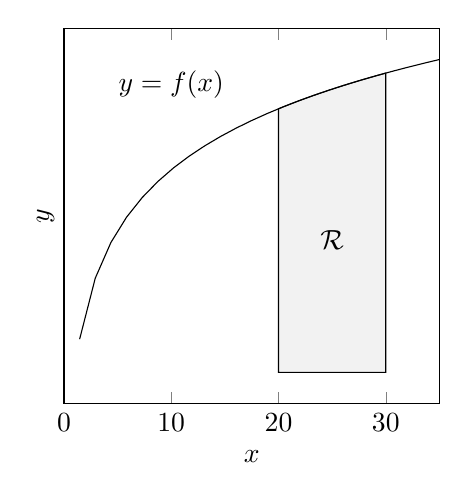
\begin{tikzpicture} 
      \begin{axis}[ cycle list={black}, xmin=0, xmax=35, 
        width=2.5in, height=2.5in, clip=false, ytick=\empty, 
        xlabel=$x$, ylabel=$y$] 
        \addplot+[domain=20:30]{0} node [right] {\;} ; 
        \addplot+[domain=20:30, fill=lightgray, fill opacity=0.2] 
        {ln(x)} \closedcycle; 
        \addplot+[domain=0:35] {ln(x)}; 
        \node [above] at (axis cs: 10, 3) {$y=f(x)$};
        \node at (axis cs: 25, 1.5) {$\mathcal{R}$};
      \end{axis} 
    \end{tikzpicture}
\begin{enumerate}

    \item Write down the value of $\Delta x$.
    \vfill

    \answerbox[$\Delta x = \solonly{\dfrac{1}{2}}$]{.5 in}{5.5 in}
    
    \item Write down a formula for $x_k$, the right endpoint of the $k$th sub-interval.
    \vfill
    
    \answerbox[$x_k=\solonly{20+\dfrac{k}{2}}$]{.5 in}{5.5 in}
    
    \item Write down a formula for $R_{20}$ using sigma notation. 
    \vfill
    
    \answerbox[$R_{20}=\solonly{\displaystyle\sum_{k=1}^{20}f(x_k)\Delta x}$ \solonly{ or $R_{20}=\displaystyle\sum_{k=1}^{20} \ln\!\left(20 + \frac{k}{2}\right)\left(\frac{1}{2}\right)$}]{.75 in}{5.5 in}
\end{enumerate}
    
    
\end{enumerate}




\end{document}